\documentclass[11pt]{article}
\usepackage{amsmath}
\usepackage{graphicx}
\setlength{\oddsidemargin}{0.0in}
\setlength{\evensidemargin}{0.0in}
\setlength{\topmargin}{-0.25in}
\setlength{\headheight}{0in}
\setlength{\headsep}{0in}
\setlength{\textwidth}{6.5in}
\setlength{\textheight}{9.25in}
\setlength{\parindent}{4em}
\setlength{\parskip}{2mm}
\usepackage{subfiles}
\usepackage{listings}
\usepackage[svgnames]{xcolor}
\usepackage{color}
\usepackage{blindtext}
\usepackage{amsmath}
\usepackage{hyperref}
\usepackage[document]{ragged2e}
\usepackage{indentfirst}
% \usepackage[a4paper, total={7in, 10in}]{geometry}

  \lstset{language=R,
    basicstyle=\small\ttfamily,
    stringstyle=\color{DarkGreen},
    otherkeywords={0,1,2,3,4,5,6,7,8,9},
    morekeywords={TRUE,FALSE},
    deletekeywords={data,frame,length,as,character},
    keywordstyle=\color{blue},
    commentstyle=\color{DarkGreen},
	breaklines=true,
  	showstringspaces=false,
}
\title{Term Project}
\author{Parth\\
\texttt{pnshah@ucdavis.edu}\and Simerpal\\
\texttt{sswhala@ucdavis.edu}\and Brian\\
\texttt{ccblai@ucdavis.edu}\and Claire\\
\texttt{chcwong@ucdavis.edu}}

\begin{document}

\maketitle

\section*{{\LARGE\bfseries Problem A}}

\begin{center}
{\LARGE\bfseries The Sky Is Not the Limit: Multitasking Across GitHub Projects}

Parth Shah
\vspace{1cm}  
\end{center}
\subfile{parth.tex}

\begin{center}
{\LARGE\bfseries Middle Cerebellar Peduncle Width - A Novel MRI Biomarker for FXTAS?}

Claire Wong
\vspace{1cm}  
\end{center}
\subfile{claire.tex}

\begin{center}
{\LARGE\bfseries Pair-Bonded Relationships and
Romantic Alternatives: Toward an
Integration of Evolutionary and
Relationship Science Perspectives}

Simerpal Whala
\vspace{1cm}  
\end{center}
\subfile{SimerpalPartA.tex}

\section*{{\LARGE\bfseries Problem B}}

\noindent{\textbf{\LARGE{Introduction}}}\\ 

\noindent{\textbf{\large{Database \(train.csv\)}}}\\

\par
	In section B of the term project, we were given a data set of Porto taxi trips \(train.csv\).
 The dataset was based off of 448 Taxis in the city of Porto, Portugal. The data was split among 9
 categories: TRIP\_ID, CALL\_TYPE, ORIGIN\_CALL, ORIGIN\_STAND, TAXI\_ID, TIMESTAMP, DAYTYPE, MISSING\_DATA,
 POLYTIME and consisted of 1710669 objects sized at 1.94 GB. The TRIP\_ID was a unique identifier for
 every trip and TAXI\_ID was a unique identifier for the taxi driver who performed the trip. CALL\_TYPE
 identified the method used to call the taxi: \textsc{\char13}A\textsc{\char13} represented a call from central,
 \textsc{\char13}B\textsc{\char13} represented if the taxi driver was demanded at a specific stand, and 
 \textsc{\char13}C\textsc{\char13} represented every other call type. ORIGIN\_CALL represented the phone number of the customer who
 demanded the taxi $($ Sets CALL\_TYPE to \textsc{\char13}A\textsc{\char13}$)$. ORIGIN\_STAND gives each taxi
 stand a unique identifier $($Sets CALL\_TYPE to \textsc{\char13}B\textsc{\char13}$)$. TIMESTAMP shows the unix
 Timestamp of the start of the trip. DAYTYPE represents the type of day it is at the start of the trip: \textsc{\char13}B
 \textsc{\char13} being a holiday or special day, \textsc{\char13}C\textsc{\char13} being the day before a type
 \textsc{\char13}B\textsc{\char13} day, and \textsc{\char13}A\textsc{\char13} being everything else.Lastly,
 POLYLINE contains a set of arrays of two elements of global coordination: the longitude and latitude.\\

\noindent{\textbf{\large{Dealing with a massive dataset}}}\\
\par
	 In order to use the dataset, we had to import it into our R data table which at first we did by using the read$()$
 function. This created an issue because the data set was taking too long to load in and often times crashing the
 IDE due to insufficient memory. A temporary fix we decided to use was to only pass in 1000 rows of the full data 
 set. This allowed us to get past the issues of read$()$ and start working on the tasks in part B. In order to fully
 fix this problem and use the entire data set we decided to use fread$()$from the data.table library. This allowed
 us to read the data set faster and use less memory.\\

\noindent{\textbf{\large{Tasks to solve}}}\\
\begin{itemize}
	\item Find density models that accurately represented the trip duration and the time when the driver was busy.
	\item Explore if the CALL\_TYPE had an effect on the meantime of taxi trips
	\item Create models that predicted trip times, distances, …$($Add other explicit models$)$
	\item Compare how those predictive models relate to one another.
\end{itemize}

\noindent{\textbf{\large{Language and Libraries used}}}\\
\par To solve these tasks our group used R to code the entire project as specified in the instructions.
 We also used the following libraries throughout the project

\begin{itemize}
	\item Devtools: Used to assist in the installation of Regtools later in the project.
	\item Dplyr: Utilized this library to create and edit data frames.
	\item Data.table: Primarily used for fread$()$ in order to speed up reading of \(train.csv\).
	\item Regtools: Allowed us to utilize many machine learning models
\end{itemize}

\noindent{\textbf{\LARGE{Exploring the possibility of trip duration}}}\\ 
\noindent{\textbf{\large{The trip duration in this database}}}\\
\par
Since POLYLINE represents a set of coordinates recorded every fifteen seconds since the start of the trip,
 The duration of a trip can be interpreted as the number of intervals existing in the set. In terms of calculation,
 letting $N_i$ donates to the number of intervals in $i^{th}$ set, The duration of $i^{th}$ trip in second is
\begin{equation}
T_i = 15(N_i -1)
\end{equation}
\par
To be more general, we convert the duration into minutes by dividing it by 60.\\

\noindent{\textbf{\large{The probability family of distribution of trip duration:}}}\\
\par
Now we have a column called trip duration, so we use hist to plot the trip duration into a histogram with the x-axis
 as the trip duration and the y-axis as the density. The probability of trip duration is found to be a gamma
 distribution family in the interval [0, 970], but because most of the time is distributed within the [0,20],
 which makes the original histogram hard to be observed, we shrink the range of x-axis to [0, 100]. However,
 the gamma distribution seems to only exist in [1,100] because the probability that the trip time is under a minute
 is too high to fit into the gamma distribution.

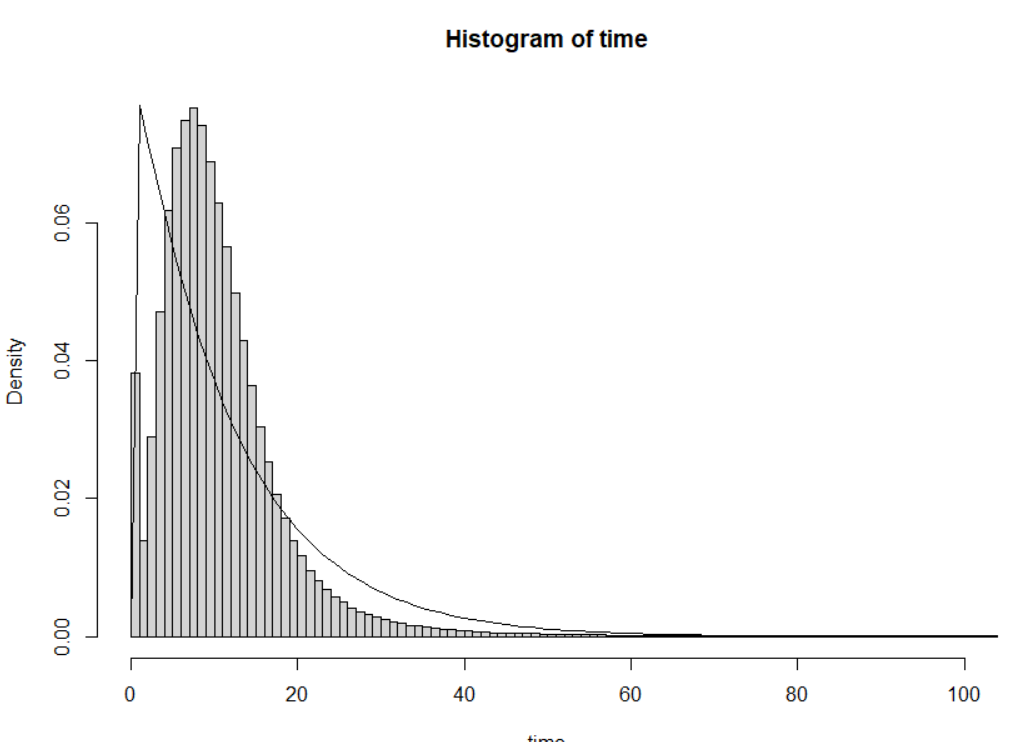
\includegraphics[scale = .5]{hist_p1_1.png}\\


\noindent{\textbf{\large{Verify the hypothesis:}}}\\
\par
To test whether the probability density of trip duration is the gamma family of distribution, we apply the actual
 curve of the gamma distribution. Therefore, we need to find the r and lambda value using mean and variance, and
 the mean and variance of time duration are found to be approximately 11.57 and 130.13, and r and lambda are found
 to be 1.0294 and 0.0889. However, the gamma distribution curve does not fit the histogram so much,  r value seeming
 to be too small. 


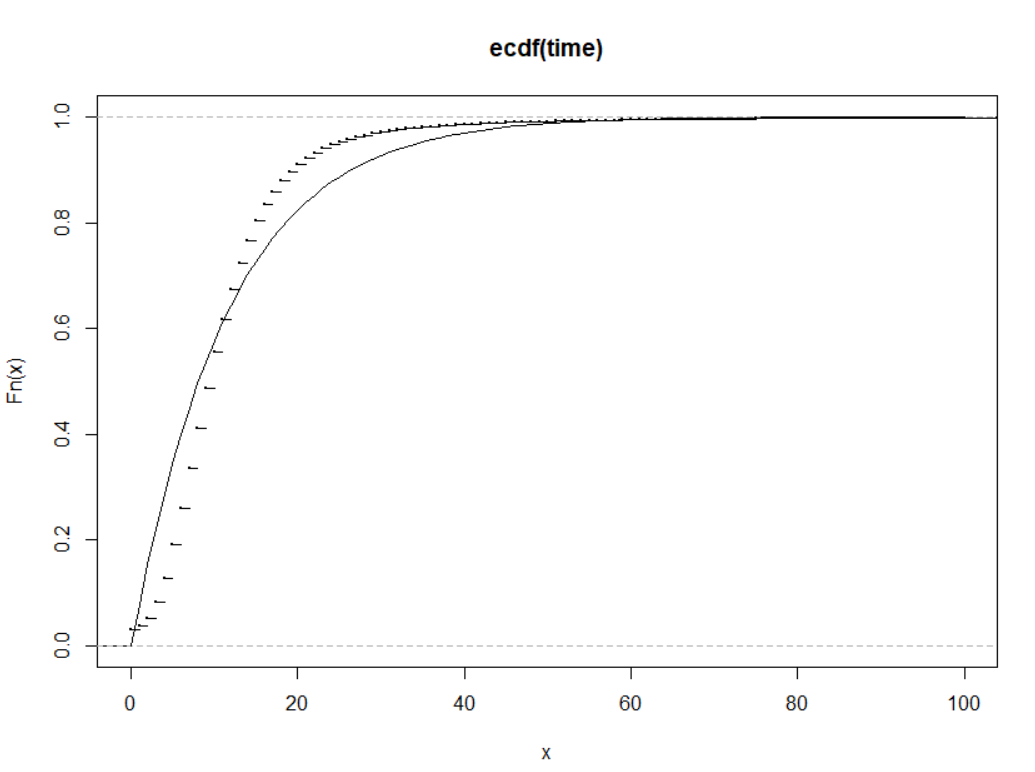
\includegraphics[scale = .50]{cdf_p1_1.png}

\par
Then, We compare the empirical cdf of T with the cdf of gamma distribution with r and lambda which we just found.
 However, they don’t match well either. \\

\noindent{\textbf{\large{First Correction}}}\\
\par
Since the proportion that the time duration is under one minute is too high, we decide to exclude it from the dataset
 and get a more rational look in the histogram. Then, we get the new mean, variance, r, and lambda,10.94, 129.88,
 1.029, and 0.0889. The new gamma distribution curve turns out to be more inaccurate, but the slope is actually a
 little bit similar to the histogram's downward slope. When we compare the empirical cdf with the cdf of our new
 database and new gamma distribution, the difference between them is not smaller than the original difference.\\
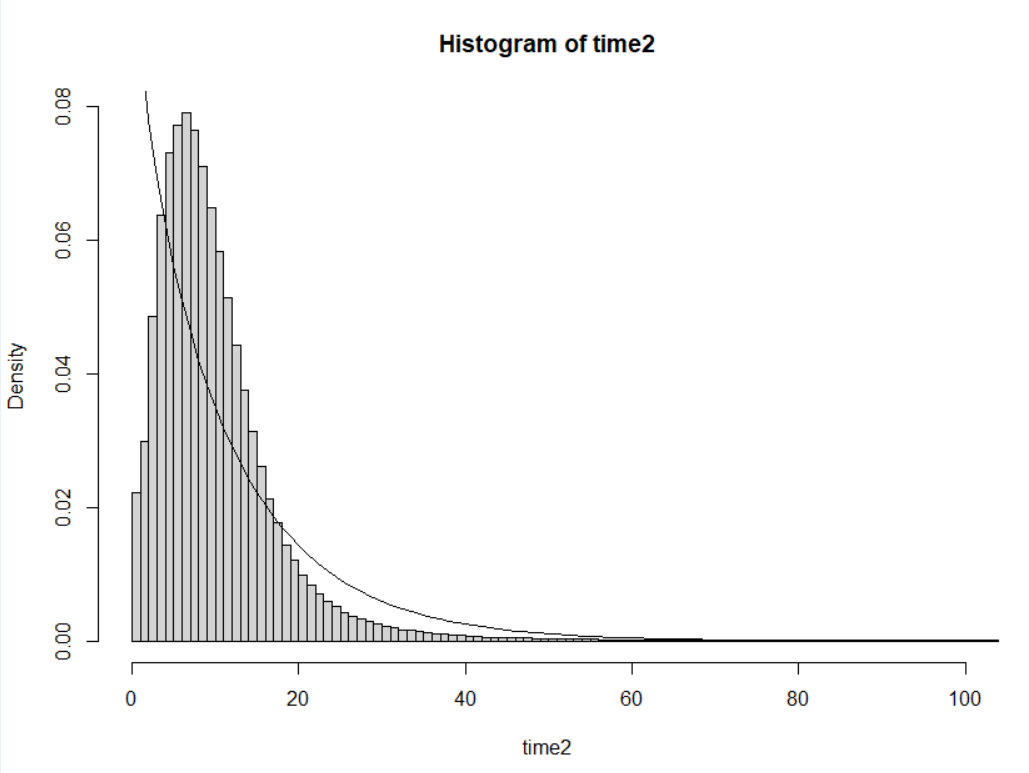
\includegraphics[scale = .30]{hist_p1_2.png}
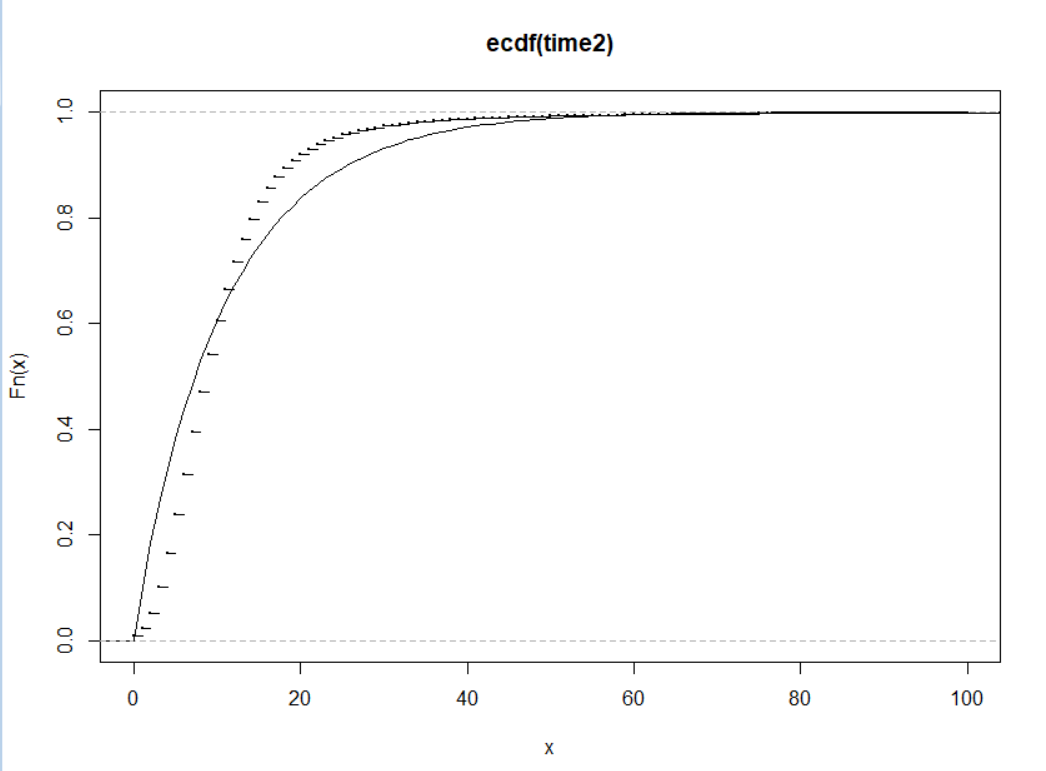
\includegraphics[scale = .30]{cdf_p1_2.png}\\


\noindent{\textbf{\large{Second Correction}}}\\
\par
The unsuccess of fitting a gamma distribution curve to the histogram is due to the high value of variance,
 which is 130 for the distribution excluding the aberrantly high proportion, that yields a small r. In fact,
 the support of T could be any value less or equal to 970, and that can lead to a very large variance with
 respect to the concentrated proportion [0,20]. With a large value of r, gamma distribution turns out to be
 steep and inaccurate; therefore. We decide to shrink the range to [1,61] by excluding every other value from
 the vector, and that forms a smaller mean and much smaller variance, 10.39 and 51.56, which yields a larger
 r and lambda, 2.09 and 0.201. Adding the curve, it fits much closer; comparing both empirical cdf and cdf of
 the gamma distribution, the result, as expected, comes up ideally. Therefore, we can confidently say the density
 of probability of trip time is the distribution of the gramma family since the proportion of interval [1,61]
 occupies 96.4\% out of all distribution.\\

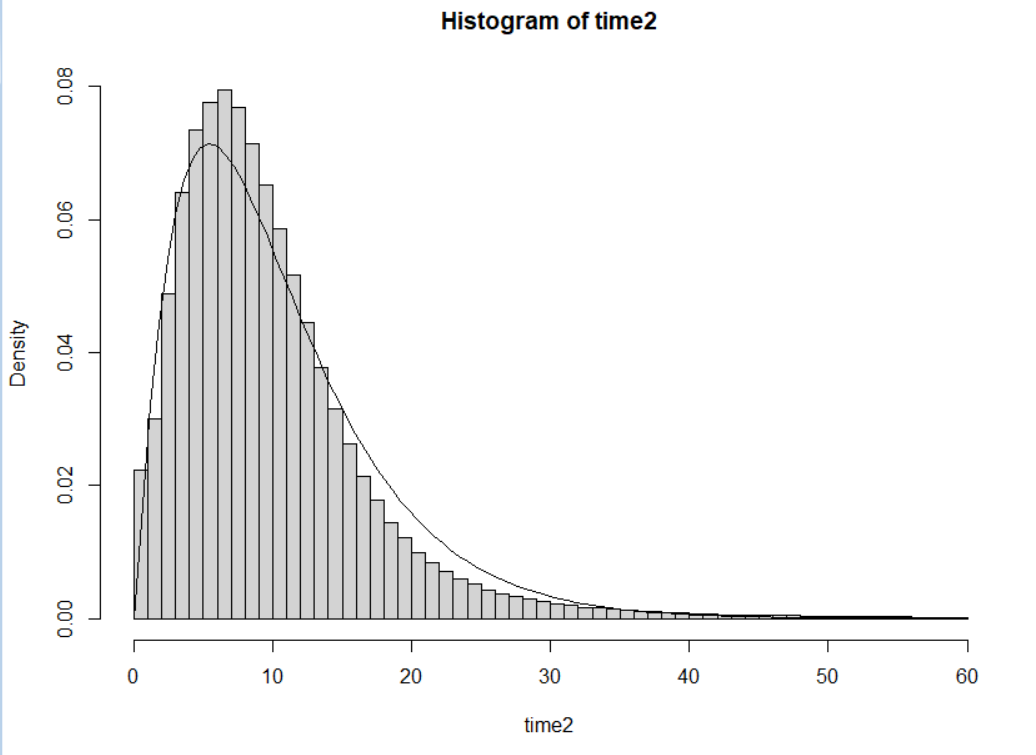
\includegraphics[scale = .50]{hist_p1_3.png}\\
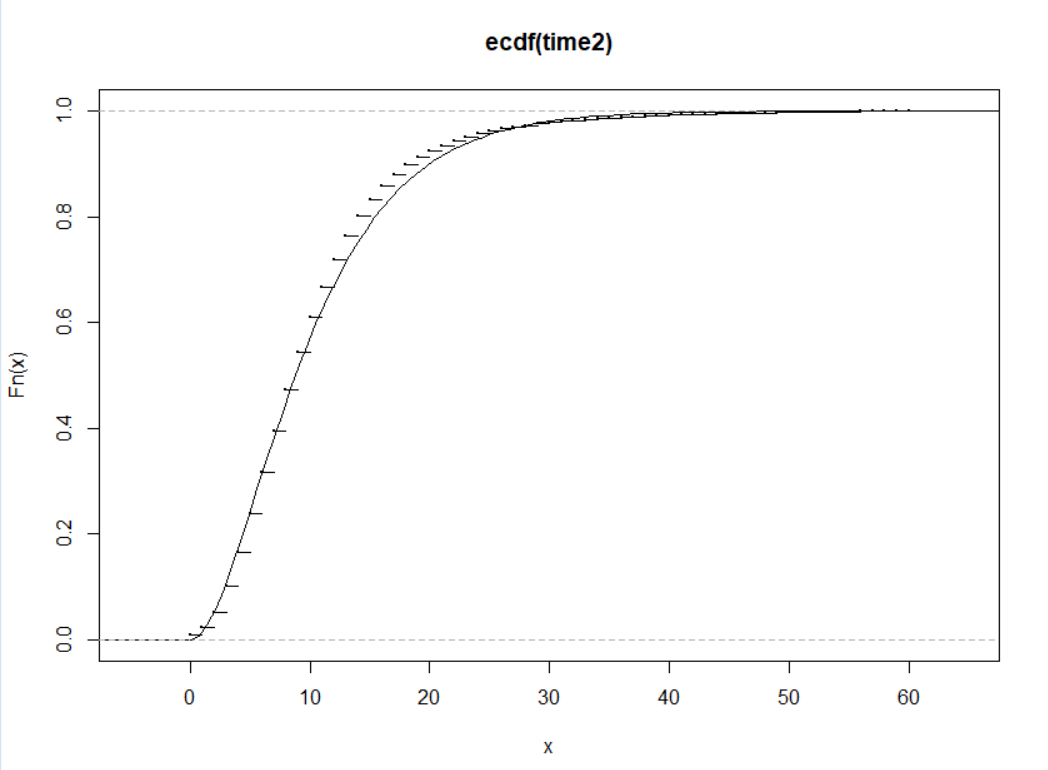
\includegraphics[scale = .50]{cdf_p1_3.png}\\

\par
The trip duration shows that people averagely take about 11 minutes to their destination but most likely within
 20 minutes. Because most of the probability, about 95\%, is distributed in [0,25].
\par
The extremely high proportion of trip duration being under one minute may be caused by human errors and instrument
 errors: drivers mistakenly or accidentally press the in-operation button, passengers' instantly calling it off,
 and technique issues. We observe that many POLYLINE don't have value, which explains that the coordination
 recorder doesn't work correctly in some cases. 

\noindent{\textbf{\large{Exploring the distribution of proportion of driver is busy:}}}\\
\textbf{Definition of Busy:}

\par
Literally, drivers being busy means they are working, but in order to calculate the proportion of drivers being busy, we also need to know when they are not busy, waiting for passengers or including they time are are off work, We assume that taxi drivers don’t have specifical time to work and amount of operating time, so we decide to define the total time as ones career life recorded in the database, from the beginning of a driver’s first trip to the ending time of his last trip. Since each driver has an unique id number, we can track the sum of trip duration as the total working time 
of $i^{th}$ driver, denoting as $U_{i}$, and Let $T_i$ denotes to the total time of $i^{th}$ driver, $R_{i_j}$ denotes to the $j^{th}$ trip duration of the $i^{th}$ driver, $N_i$ denotes to the number of trips $i^{th}$ driver have completed, and $B_i$ denotes to the proportion of time $i^{th}$ driver being busy; the time can be calculated as

\begin{equation}
T_i =TimeStamp_{i last}-TimeStamp_{i first} +R_{iN_i}
\end{equation}

\par
The busy time is as

\begin{equation}
U_i = \sum_{k=1}^{N_i} R_{ik}
\end{equation}

\par
Then, the proportion is

\begin{equation}
B_i = \frac{U_i}{T_i}
\end{equation}

\textbf{Probability Distribution:}
\par
Plotting B into the histogram, we get an approximate normal distribution in the range of (0,0.23]. As we observe there are some extreme cases that drivers only work about 0.005 of their time involved in this career, averagely 0.12 hour a day.

\noindent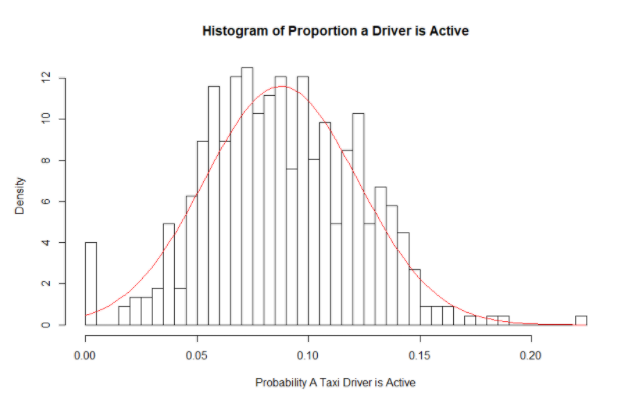
\includegraphics{Hist(PropActDriv).png}\\

\noindent{\textbf{\LARGE{Investigation of average trip times using CALLTYPE:}}}
% \centering\noindent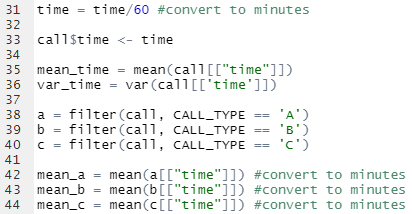
\includegraphics{Part3(Code).png}\\
\begin{lstlisting}
callSplit <- split(trainData, trainData$CALL_TYPE)

i <- 1
res <- list()
for (call in callSplit) {
	res[[i]] <- apply(call, 1, getDur);
	i <- i + 1
}
  
print(paste0('A: mean: ', mean(res[[1]]), 'var: ', var(res[[1]])))
print(paste0('B: mean: ', mean(res[[2]]), 'var: ', var(res[[2]])))
print(paste0('C: mean: ', mean(res[[3]]), 'var: ', var(res[[3]])))
\end{lstlisting}

\flushleft\par
In order to obtain the trip times we took the length of the POLYTIME and multiplied it by 15 to obtain how many seconds a trip took. This was then divided by 60 to get the time in minutes.

\par
We filtered the original dataset to contain only the CALL\_TYPE column and appended our time column to this new dataset. We then applied the mean() and var() functions to the newly converted minutes variable to obtain the mean and variance of the time.

\par
General Dataset Mean (TIMESTAMP):

\begin{equation}
Mean (Overall) = \frac{Minutes (Converted)}{1710660} = 12.201
\end{equation}

\par
On the other hand, to get the values with the dependency of CALLTYPE, we used filter() to sort through the data in order to get the correct TIMESTAMP values in regard to the three CALLTYPE’s A,B, and C. After we used mean() to get a mean of the TIMESTAMPS sorted by CALLTYPE. 

\begin{equation}
Mean (CALLTYPE = A) = \frac{Minutes (Converted)}{1710660} = 12.511
\end{equation}

\begin{equation}
Mean (CALLTYPE = B) = \frac{Minutes (Converted)}{1710660} = 11.086
\end{equation}

\begin{equation}
Mean (CALLTYPE = C) = \frac{Minutes (Converted)}{1710660} = 12.873
\end{equation}

\noindent{\textbf{\large{Verification: }}}
\par
In order to see whether the means change with the different call types, let's check the 95\% confidence interval of each mean:
\begin{equation*}
	\begin{aligned}
		Mean (CALL TYPE) &&Interval\\
A:  && 12.478 \le \mu \le 12.533\\
B:  && 11.069 \le \mu \le 11.103\\
C:  && 12.829 \le \mu \le 12.917\\
	\end{aligned}
\end{equation*}
\par
Where $\mu$ is the mean. From here, we can say we are 95\% confident that the true mean of trip time for the call type of A falls 
within the confidence interval range of A, the true mean of trip time for the call type of B falls within the confidence interval 
range of B, and the true mean of C falls within the confidence interval range of C.

\noindent{\textbf{\large{Analysis: }}}
\par
Difference between trip times using different call types:

\begin{equation}
Call Type A = 11.940 - 12.506 = -0.566 (33.96 Seconds Slower)
\end{equation}

\begin{equation}
Call Type B = 11.940 - 11.086 = 0.854(51.24 Seconds Faster)
\end{equation}

\begin{equation}
Call Type C = 11.940 - 12.873 = -0.933 (55.98 Seconds Slower)
\end{equation}

\begin{equation}
Call Type C > Call Type A > Call Type B
\end{equation}

\par
In general, the type of call made to summon a taxi doesn’t make much of a difference in regards to trip time, but the fastest would be from a 
specific stand. Furthermore, we can examine the variance of each call type to determine the spread of the data set compared to the mean.

\begin{equation}
Variance (Overall) = 130.24
\end{equation}

\begin{equation}
Variance (Call Type A) = 72.26
\end{equation}

\begin{equation}
Variance (Call Type B) = 64.76
\end{equation}

\begin{equation}
Variance (Call Type C) = 269.50
\end{equation}

\par
The Variance of the 3 Call Types are fairly close with the exception of Call Type C. This indicates that there is a lot of volatility in the trip times for Call Type C. 
This could be caused by the fact that Call Type C is the least specific of the three call types, taking riders from various methods instead of a set way of getting riders. 
Further, there are many explanations as to why the different call types have different mean trip times. As Call Type ‘C’ has the greatest variance, it can be inferred that 
most of the longer trip times had Call Type ‘C’. This is shown below:
\begin{equation*}
	\begin{aligned}
		Max(Overall) =&& 970\\
Max(Call Type A) =&& 580.75\\
Max(Call Type B) =&& 958.75\\
Max(Call Type C) =&& 970
	\end{aligned}
\end{equation*}

\par
We also find that there is only 1 entry with Call Type 'A' with a time greater than 500 minutes. For Call Type 'B', there are 6, and for Call Type 'C', there are 38. 
This could be explained by a difference of dataset numbers. So the percentages were calculated, and it was found that 0.000274 \%, 0.000734 \%, and 0.00720 \%

\noindent{\textbf{\LARGE{Moddling the Data}}}\\
\textbf{Models:}
\par
In the term project we decided to use the following models to visualize our data:
\begin{itemize}
	\item Linear
	\item Linear Polynomial
	\item k-Nearest Neighbors
	\item Boosting
\end{itemize}

\textbf{Moddling Distance and Speed:}
\par
The first model we decided to take on was modeling the distance vs the 
speed. In order to plot these two variables on a model we had to obtain 
the distance and speed. The distance we obtained by utilizing the 
coordinates from POLYLINE column in the dataset. After we just took the 
start and end points of the formula and applied the Haversine distance 
formula. The Haversine (or great circle) distance is the angular distance 
between two points on the surface of a sphere. It is a very accurate way 
of computing distances between two points on the surface of a sphere using 
the latitude and longitude of the two points.
\begin{equation*}
	\begin{aligned}
		(x1,y1) &&= Starting Coordinates\\
		(x1,y1) &&=Ending Coordinates
	\end{aligned}
\end{equation*}

\par
In order to figure out the average speed we now have distance and can obtain time elapsed during a trip by figuring out trip duration. In order to figure out trip duration we took the length of the POLYLINE variable where each length represents 15 seconds. So, we used the following formula:

\begin{equation*}
	Speed = \frac{Distance} {Length(POLYLINE) * 15 / 60}
\end{equation*}

\textbf{Moddling Time:}
\par
Looking for other parameters, we decided to check if using the day of the year and time of the day affect the accuracy of the predictions. In order to get this data, we use the timestamp and convert it to a DayTime using

\begin{lstlisting}
as.POSIXct(date_ref$TIMESTAMP, origin = "1970-01-01")
\end{lstlisting}
\par
Next, we extract the Date, Day of the year, hour, minute and second from that
\begin{lstlisting}
date_ref$DATE <- format(test, format = "%Y-%m-%d")
date_ref$DAY_OF_YEAR <- as.integer(format(test, format = '%j'))
date_ref$HOUR <- as.integer(format(test, format = "%H"))
date_ref$MIN <- as.integer(format(test, format = "%M"))
date_ref$SEC <- as.integer(format(test, format = "%S"))
\end{lstlisting}

\par
Now that we have the essential data, we can create 2 variable to use for our predictions, 
\begin{lstlisting}
time <- (date_ref$HOUR * 60 + date_ref$MIN + date_ref$SEC / 60)
dyear <- data.frame(date_ref$DAY_OF_YEAR + time / 24)  
\end{lstlisting}

\par
In short, the time of day was calculated by extracting the hour, minute, and second (eg. 00:00:00) from the Unix timestamp in the TIMESTAMP column of the dataset. Then, the hour was added to the minutes/60 plus the seconds /3600. Divisions were done to convert the time into hour.

\par
Thus, in a 24 hour day, 0 is midnight and 23.99 is right before midnight of the same day. For the time of day predictions, no distinctions were made on the day of the year, only the time of day. 
\par
For the day of the year, the date (eg 01/01/2013) was extracted from the Unix timestamp and was converted into the day of the year, where 01/01/2013 is day 1 and 12/31/2013 is day 365. 

\textbf{Moddling Call Type:}
\par
Since we were talking about call types affecting the duration, we decided to use them in order to increase the prediction accuracy. Since there can be only A,B or C type, we can convert them to 1,2 or 3 so that we can directly feed it to the model.

\begin{lstlisting}
call <- apply(trainData, 1, function(row) {
	return(as.integer(charToRaw(row[[2]]))-64)
})
\end{lstlisting}

\noindent{\textbf{\LARGE{Predictions and Parameters}}}\\
\par
In the prediction part of modeling we decided we will be predicting the time duration of a trip depending on multiple factors. The 3 different sets of parameters we decided to use:
\begin{itemize}
	\item Predict Time Duration using Distance only
	\item Predict Time Duration using Speed and time of the day only
	\item Predict Time Duration using Distance, Speed, Time, and Type of Call
\end{itemize}

\noindent{\textbf{\LARGE{Analysis}}}\\
\par
\textbf{Predict Time Duration using Distance only}
\par
We found that this gave us really good results up to an extent with the density curves somewhat going along the actual values.

\textbf{Predict Time Duration using Speed and time of the day only}
\par
We found that this results in a really bad prediction since the speed and time of day alone cannot really predict the duration of the trip. We can see in the density graphs that this no way resembles the actual data.

\textbf{Predict Time Duration using Distance, Speed, Time, and Type of Call}
\par
This gave us the most accurate results with the KNN model almost exactly coinciding with the actual data. We deciphered that giving the model more parameters to train on, the model can correlate more values and thus can give us better predictions.

\noindent{\textbf{\LARGE{Confidence Interval for Linear model}}}\\
\par
To find the confidence interval for the linear model, we first had to find the $q_{\alpha/2}$ values. We found them by using the qgamma function with the rate and shape same as those of the actual data and p as 0.025.
\begin{lstlisting}
z = qgamma(0.025, mean(actual$dur) ^ 2 / var(actual$dur), 
    mean(actual$dur) / var(actual$dur))
\end{lstlisting}
\par
Now the next step was to find the standard error which can be found using a simple formula.
\begin{lstlisting}
se = sqrt(sum((actual - prediction) ^ 2) / n)
\end{lstlisting}
Now that we have both, the z and se, we can find the intervals as $T \pm q_{\alpha/2} s.e.(T)$

\appendix
\section*{Appendix}
\lstinputlisting[language=R]{TermProject.R}
\end{document}